\documentclass[a4paper]{article}
\usepackage{latexsym}
\usepackage[a4paper]{geometry}
\usepackage{color}
\usepackage{listings}
\usepackage[pdftex]{graphicx}
\usepackage{subfig}

\definecolor{Blue}{rgb}{0,0,0.5}
\definecolor{Green}{rgb}{0,0.75,0.0}
\definecolor{LightGray}{rgb}{0.6,0.6,0.6}
\definecolor{DarkGray}{rgb}{0.3,0.3,0.3}
\lstset{language=Matlab,
   keywords={function,uint8,uint16,uint32,double,break,case,catch,continue,else,elseif,end,for,global,if,otherwise,persistent,return,switch,try,while},
   basicstyle=\ttfamily\small,
   breaklines=true,
   keywordstyle=\bfseries\color{Blue},
   commentstyle=\itshape\color{LightGray},
   stringstyle=\color{Green},
   numbers=left,
   numberstyle=\tiny\color{DarkGray},
   stepnumber=1,
   numbersep=10pt,
   backgroundcolor=\color{white},
   tabsize=2,
   showspaces=false,
   showstringspaces=false,
   captionpos=b}

%Boldface text for type writer font
\usepackage{bold-extra} %\DeclareFontShape{OT1}{cmtt}{bx}{n}{<5><6><7><8><9><10><10.95><12><14.4><17.28><20.74><24.88>cmttb10}{}

%Break words properly at the end of a line (which isn't sloppy...)
\sloppy

%Use command \exercise for each exercise
\newcounter{exerciseCount}
\setcounter{exerciseCount}{0}
\newcommand{\exercise}[1]{\addtocounter{exerciseCount}{1} \noindent \medskip {\large \textsf{\textbf{Exercise \arabic{exerciseCount} \--- #1}}} \par}
\renewcommand{\theenumi}{\textsf{\textbf{\alph{enumi}}}}

%Use command \code for code snippets
\newcommand{\code}[1]{\textnormal{\texttt{#1}}}



\title{\textsf{Image Processing \\ lab 1}}
\author{Mattijs Meiboom (s1398342)}
\date{\today}

\begin{document}
\maketitle

\exercise{Reducing the number of intensity levels}
\begin{enumerate}
\item
The intensity levels in our 8-bit image are represented on a scale of 0-255 and we thus have 256 levels of intensity. To resample the image to a fewer number of levels, we will take the following steps.
	\begin{enumerate}
		\item First we convert the image-representation to use floats on the interval [0,1]
		\item We then determine the size of each level (delta, by dividing [0,1]  by the number of levels)
		\item For each pixel in the image, we determine in which level the value falls (by dividing by our delta)
		\item Finally, we map each level to a value in the domain [0,255]
	\end{enumerate}
\lstinputlisting{../../ipreduce.m}

\item
\begin{center}
\begin{tabular}{cccc}
    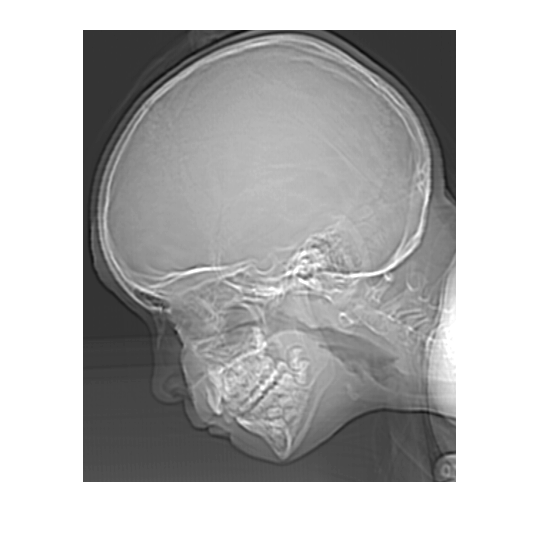
\includegraphics[width=0.2\textwidth]{../11_skull.png} &
    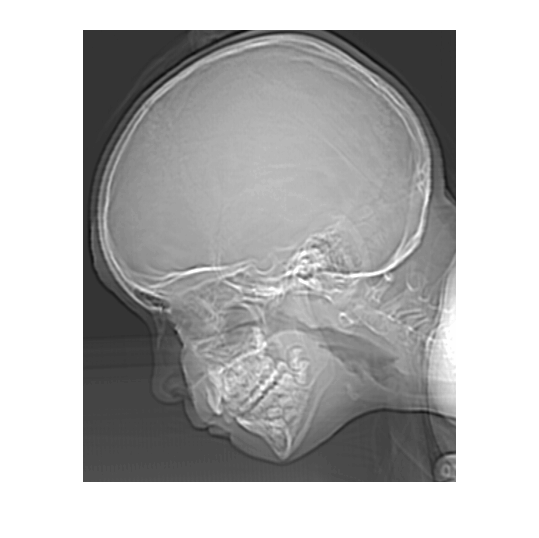
\includegraphics[width=0.2\textwidth]{../11_skull_k7.png} &
    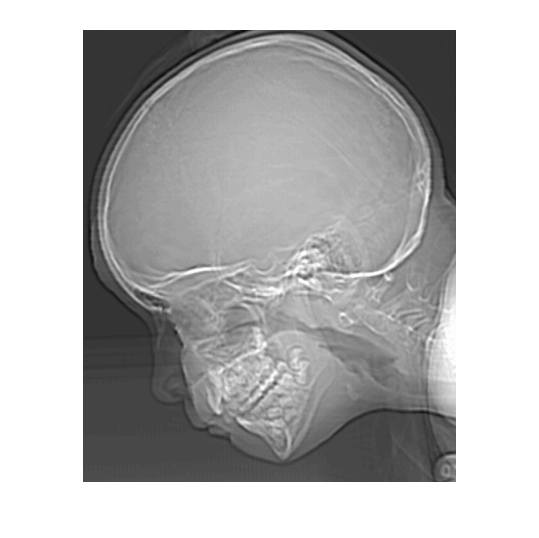
\includegraphics[width=0.2\textwidth]{../11_skull_k6.png} &
    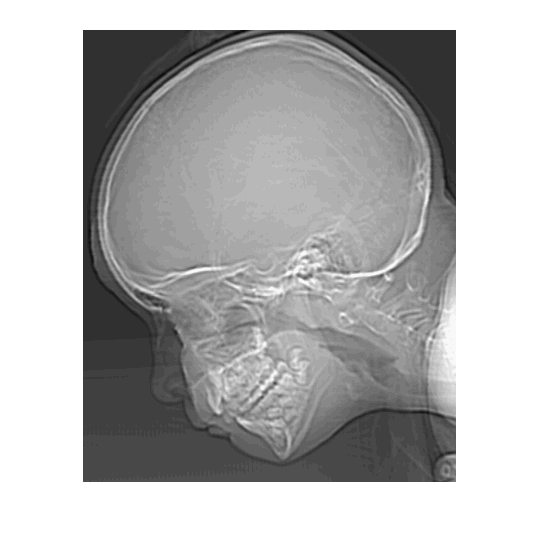
\includegraphics[width=0.2\textwidth]{../11_skull_k5.png}\\
    256 levels & 128 levels & 64 levels & 32 levels \\
    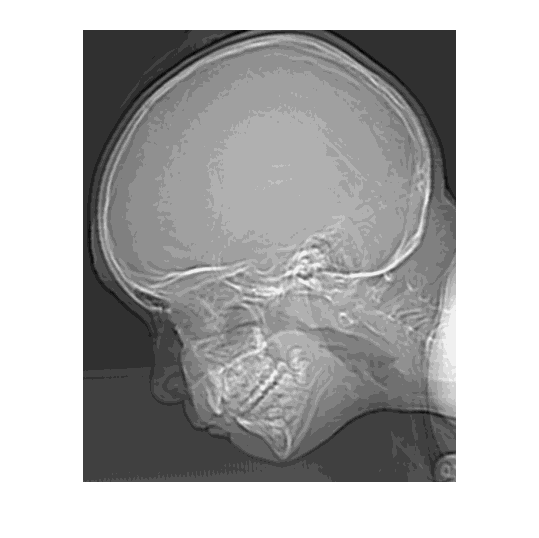
\includegraphics[width=0.2\textwidth]{../11_skull_k4.png} &
    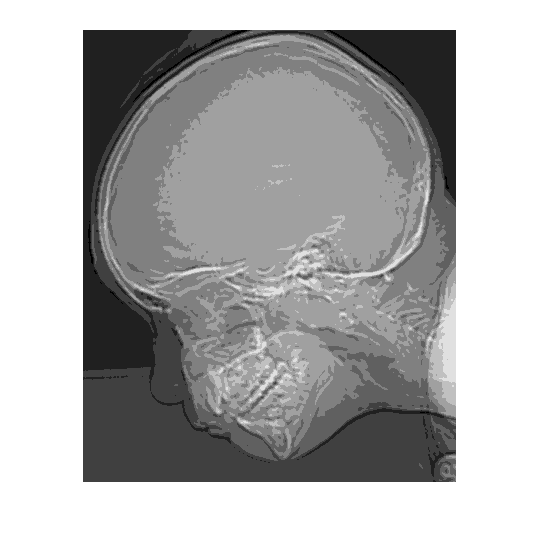
\includegraphics[width=0.2\textwidth]{../11_skull_k3.png} &
    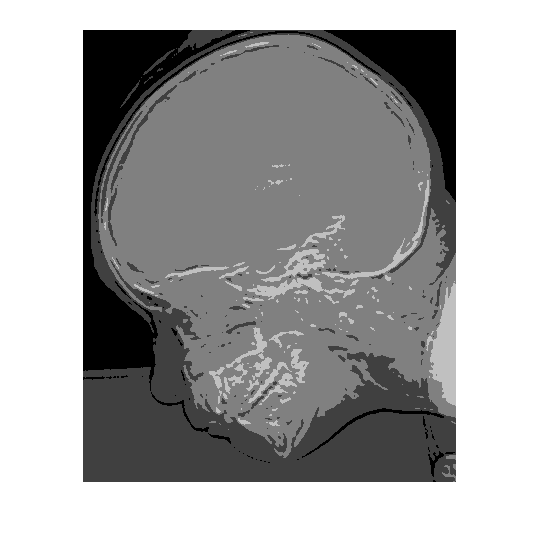
\includegraphics[width=0.2\textwidth]{../11_skull_k2.png} &
    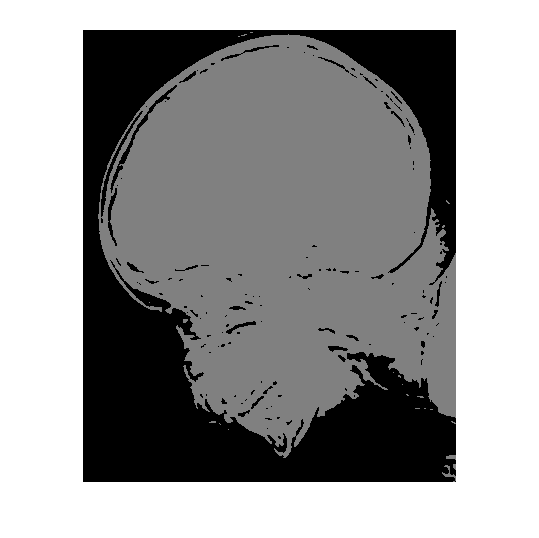
\includegraphics[width=0.2\textwidth]{../11_skull_k1.png}\\
    16 levels & 8 levels & 4 levels & 2 levels
\end{tabular}
\end{center}
\end{enumerate}


\exercise{Bilineair interpolation}
\begin{enumerate}
\item
The following is a function for scaling an image (using bilineair interpolation). To reach this result, we take the following steps. This should work for both scaling and shrinking, as it uses the ratio between source and target image.
	\begin{enumerate}
	\item First, we determine the spacing of pixels in the target image, by stretching the original in the x and y direction. 
	\item Then, using this spacing information, we obtain for each pixel in the target image a (non-discrete) position in the source image and it's position with respect to the pixels surrounding it.
	\item We interpolate the value of the target pixel by multiplying the value of and distance to the 4 surrounding pixels and summing these 4 values.
	\end{enumerate}
\lstinputlisting{../../ipresizebl.m}
\item
\begin{center}
\begin{tabular}{ccc}
    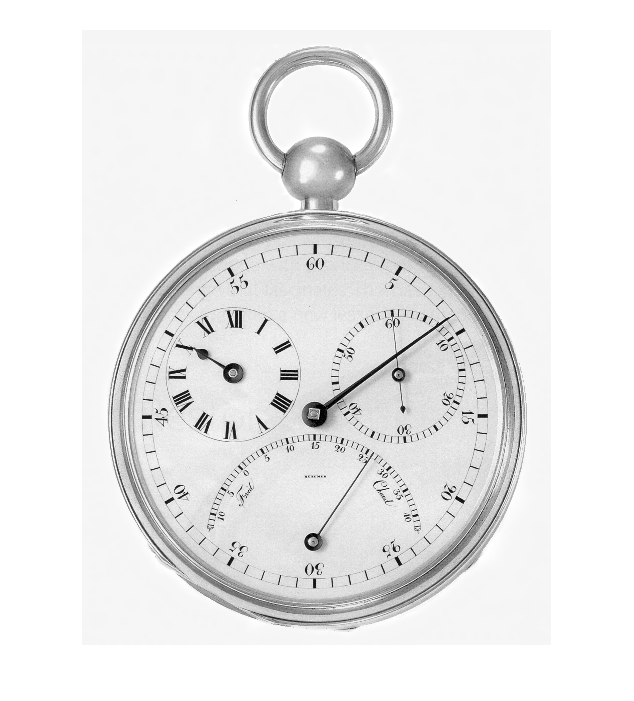
\includegraphics[width=0.2\textwidth]{../12_original.png} &
    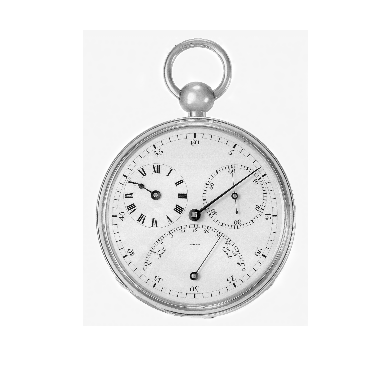
\includegraphics[width=0.2\textwidth]{../12_shrunk.png} &
    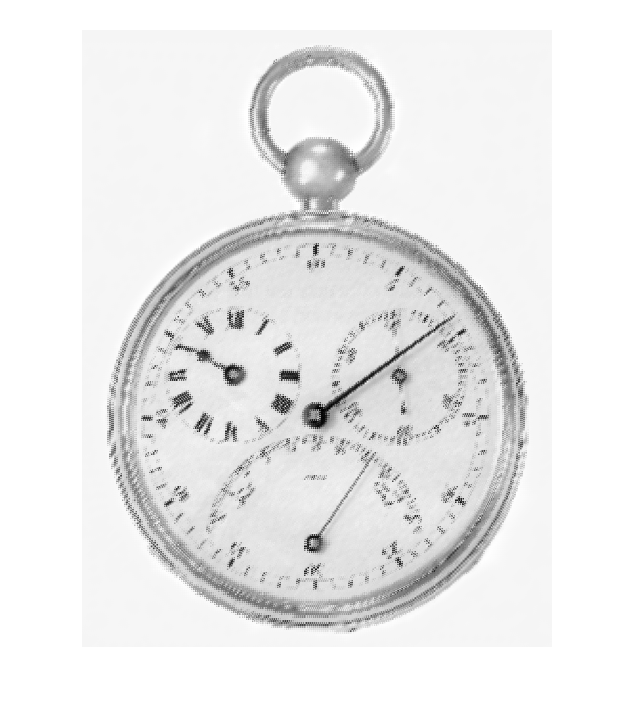
\includegraphics[width=0.2\textwidth]{../12_restored.png}\\
\end{tabular}
\end{center}
\item
When viewing the results at 100\%, you will notice that the restored image has some artifacts introduced with respect to the original image. By first shrinking the original, we loose detail in areas that have rapidly changing values (such as edges). When restoring to the original size (especially when scaling by a large factor) these areas can become jaggy due to the lineair nature of the interpolation and the lack of detailed information.
\end{enumerate}
\newpage
\exercise{Histogram equalization}
\begin{enumerate}
\item
For the histogram equalisation, we will use a transformation function which is actually a summation based on the normalized histogram of the image. This transformation has the property that for a certain intensity level r, the output of the transformation function is the probability that a pixel has intensity level equal or lower then r. This way, intensity levels are distributed as equally as possible over the domain of r. As a result, the equalized image will consist of a more distributed set of the intensity domain (unless, as in the case of our image, one value is very dominant which will then shift towards the center of the domain).
\lstinputlisting{../../iphistogram.m}
\lstinputlisting{../../iphisteq.m}
\item
\begin{center}
\begin{tabular}{ccc}
    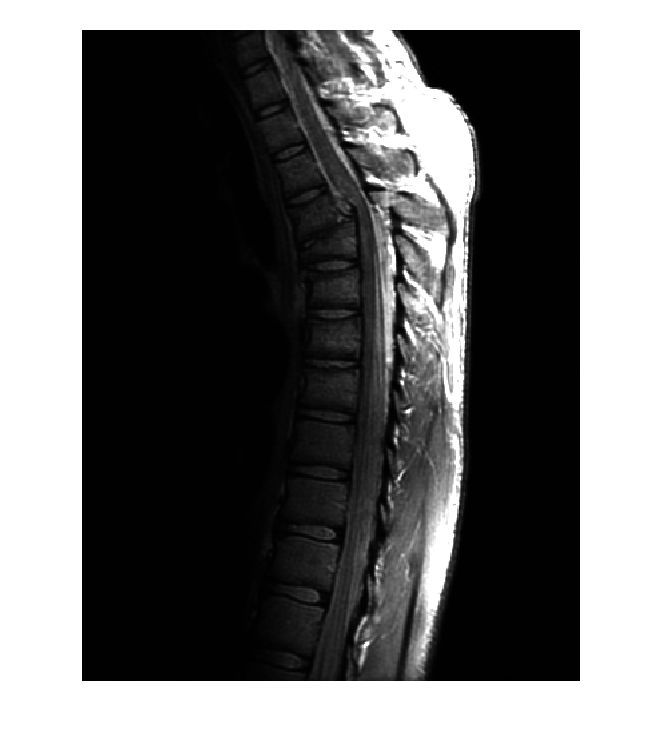
\includegraphics[width=0.2\textwidth]{../13_spine.png} &
    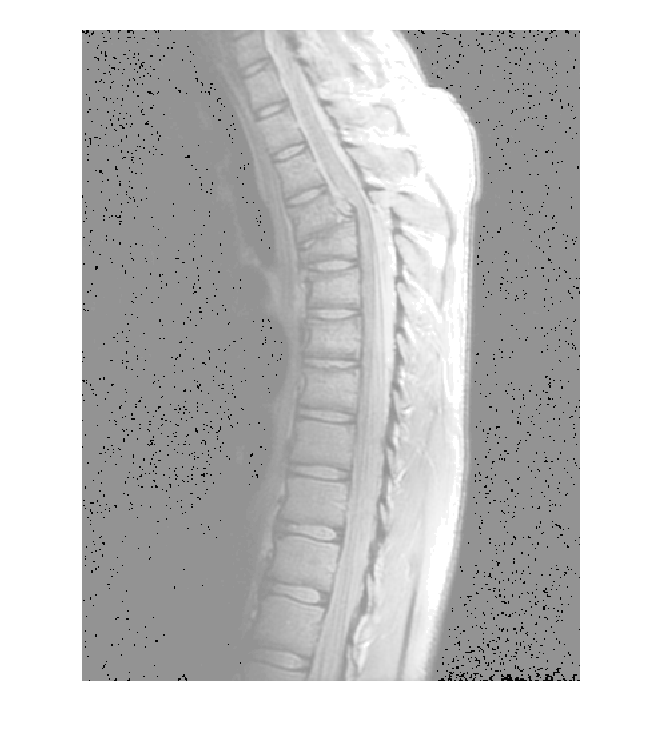
\includegraphics[width=0.2\textwidth]{../13_spine_eq1x.png} &
    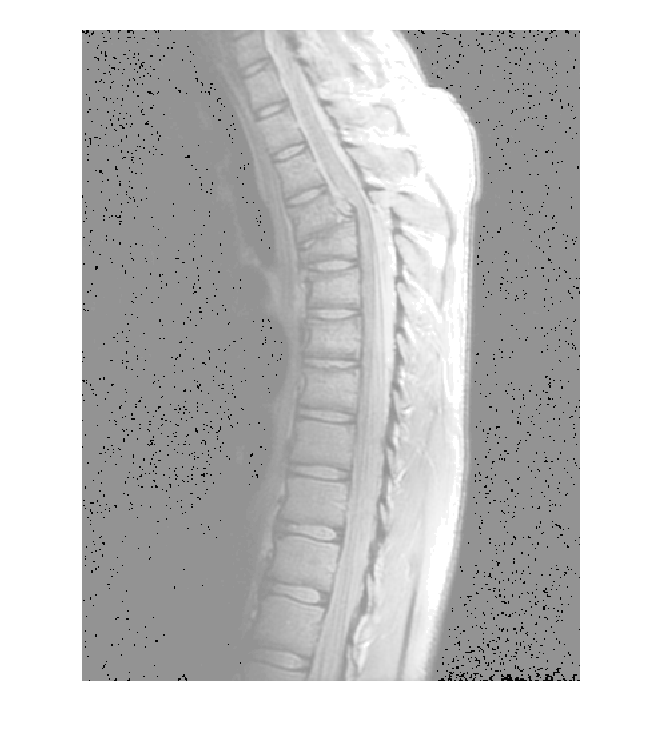
\includegraphics[width=0.2\textwidth]{../13_spine_eq2x.png}\\
    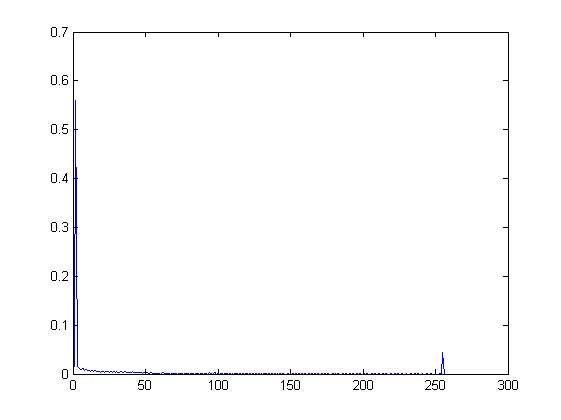
\includegraphics[width=0.2\textwidth]{../13_hist_spine.png} &
    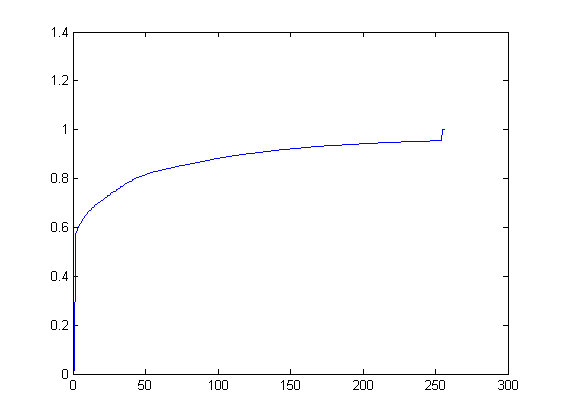
\includegraphics[width=0.2\textwidth]{../13_transformation.png} &
    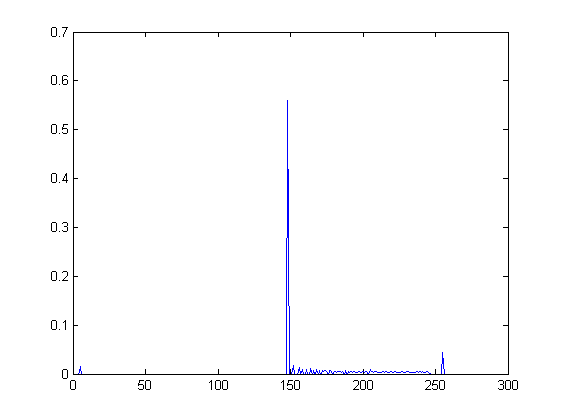
\includegraphics[width=0.2\textwidth]{../13_hist_eq.png}\\
\end{tabular}
\end{center}
\item
The reason that the result for equalizing once or twice are identical is that, in the equalized image, intensity levels have already been distributed according to the transformation function and thus when calculating a transformation for the second pass, the probability of a pixel having intensity level smaller or equal to r (r in [0..1]) is actually r.
\end{enumerate}



\end{document}
